\documentclass[letterpaper, 10 pt]{ieeeconf}
\overrideIEEEmargins

\usepackage{graphicx}

\title{\LARGE \bf Hybrid Fuels Additives}

\author{{Pablo Martinez, Nicholas Quillin, Karthik Nuti, Nashwan Chowdhury}}
\begin{document}
\maketitle
\thispagestyle{empty}
\pagestyle{empty}

\begin{abstract}
Traditionally, many fuel mixtures are made with a variety of additives in order to enhance the combustion process. This research aims to create the idealized hybrid fuel blend by testing additives to a paraffin wax fuel mixture, which will enhance the absorptivity, reactivity, and regression rate of the hybrid fuel grain.
\end{abstract}

\section{Introduction}
\label{sec:introduction}
I like trains
Recently, hybrid rocket engines (HRE) have experienced
a resurgence of popularity as a result of recent technological advances. Hybrid rocket engines combine aspects of both solid and liquid propulsion. From solid motors, they inherit a solid fuel grain which lines the combustion chamber and protects it from hot combusting gasses, and from liquids, they store the oxidizer in a separate fluid tank, allowing for control over the combustion process. Due to their safety, simplicity and throttling capability they have been chosen as the ideal system of in-house propulsion development at Aero Mavs.

\begin{figure}[h]
    \centering
    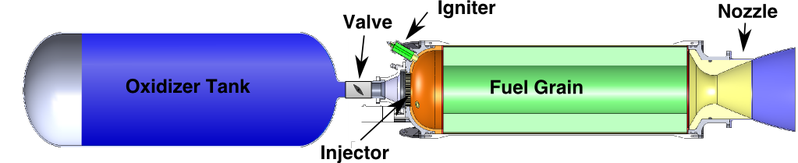
\includegraphics[width=1\linewidth]{Figures/hybridthingi.png}
    \caption{Hybrid Rocket Engine\cite{HybridImage}}
    \label{fig:placeholder1}
\end{figure}

One of the largest issues with traditional hybrid engines is their low regression rate and the secondary issues that this problem creates. Low regression rates are inherent to the way that traditional polymeric fuels combust in the combustion chamber. In a hybrid engine the combustion process takes the form of a long diffusion flame sandwiched in the turbulent boundary layer between the oxidizer plume which originates from the injector on the end of the engine, and the fuel vapor, which is typically generated from the pyrolysis/depolymerization and vaporization of the fuel grain\cite{HumbleHybrid}. Since this interface area and the heat transfer to the fuel grain is limited by the geometry, the reaction rate too is limited, leading to low regression rates compared to solid and liquid propulsion. This characteristic, in turn, introduces several problems in the practical application of hybrid engines. For instance, limited mass flow in the engine limits the total thrust an engine can produce creating scaling issues. While there are various ways to go about mitigating regression rate issues in design, they all have their own downsides, from potentially inducing combustion instability to complicating the manufacturing process or reducing the combustion efficiency. In other words any approach that can inherently increase the regression rates in hybrid fuels would greatly simplify and improve and simplify the practical design of hybrid rocket engines.

\begin{figure}
    \centering
    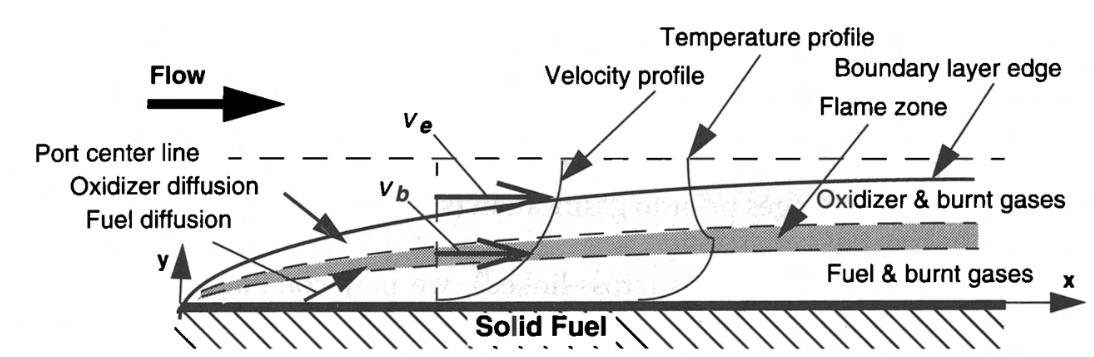
\includegraphics[width=1\linewidth]{Figures/diffusionFlame.png}
    \caption{Diffusion Flame in Hybrid rocket engine\cite{HumbleHybrid}}
    \label{fig:placeholder}
\end{figure}

The way we propose to combat this issue is to improve the reactivity of the fuel under combustion conditions. Due to the inherent safety afforded by separating the fuel and oxidizer before launch, hybrids lend themselves very well to this kind of experimentation and development. 

\section{Project Desription}
\label{sec:Project Description}
Ever since Zborwski and Muller learned by comparing the reaction rate of new cloths from used ones, that some metals acted as catalysts and helped facilitate the hypergolic combusiton\cite{ignition}, nearly all practical rocket engine designs have at least investigated additives to their propellants in order to improve system efficiency and performance. As such the goal of this research is to develop our own hybrid rocket fuel blend that will combine the characteristics of various additives to a parrafin fuel base.  

In this research we plan on testing various additives to determine their effects on the fuel grain. The most promising additives we hope to experiment are carbon-black, an agent designed to improve the conduction of radiative energy to the fuel grain by increasing its absortivity\cite{T59IREC2018}, Ferrocene in order to lower the ignition temperature and increase flame stability, and aluminum powder to increase the reactivity of propellant. 

Our plan is to first complete and light a hybrid engine testbed in October to get some baseline control data using a known fuel formulation. Then starting in January conduct a design sweep of various test samples using a taguchi orthagonal array methodology to minimize the number of tests as well as determine how the doping agents interact with one another in combination. Finally once we have determined the best configuration, use it in a full scale M-class rocket engine we propose to build and test in April.

\bibliographystyle{ieeetr}
\bibliography{references}

\end{document}

